\section{Estructura general}

    El laboratorio virtual de sistemas de control clásicos y difusos fue pensado de modo que cada una de sus funcionalidades principales sean independientes la una de la otra, no obstante, ciertas rutinas son comunes entre ellas. Por otro lado, se organizo la aplicación de modo que cada funcionalidad principal posea un archivo \enquote{handler}, el cual hará de intermediario entre la interfaz gráfica y las rutinas de calculo que se encuentran en un archivo de rutinas. La \cref{fig:estructuraMain} sirve como referencia de la estructura general utilizada.

    \begin{figure}[htb]
        \centering
        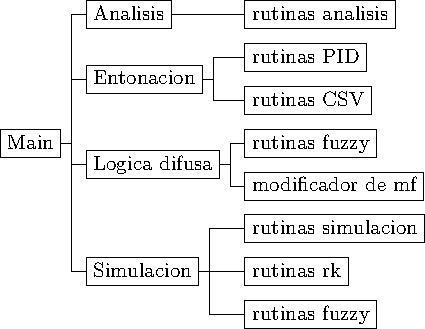
\includegraphics[width=0.8\textwidth]{estructuraMain.pdf}
        \caption[Diagrama general de la aplicación]{\textbf{Diagrama general de la aplicación}. La estructura general de la aplicación, la segunda columna representa a los archivos handler mientras que la tercera son los archivos de rutinas  Fuente: Elaboración propia.} 
        \label{fig:estructuraMain}
    \end{figure}

\section{Análisis de sistemas de control}
    
    Con esta función se quiso dar la posibilidad de realizar los análisis en el tiempo y en frecuencia típicos para un proceso ingresado por el usuario, los análisis típicos son: respuesta al escalón, respuesta al impulso, diagrama de bode, diagrama de Nyquist, lugar de las raíces y diagrama de Nichols. El \cref{code:analisis} muestra un pseudo código de la funcionalidad de análisis de sistemas de control.

    \begin{longlisting}
        \caption{Pseudo código para el análisis de sistemas de control}
        \label{code:analisis}				
        \begin{minted}[escapeinside=||,
            mathescape=true,
            autogobble=true,
            fontsize=\footnotesize,
            obeytabs=true,
            tabsize=4,
            baselinestretch=1]{text}
            |\bf{WHILE}| True: # Ciclo principal
                |$\vdots$|
                |\bf{IF}| validaciones_entradas_análisis:
                    validar_entradas_análisis()
                
                |\bf{IF}| usuario_presiona_calcular:
                    chequeo_TF_SS()
                    creación_proceso()
                    escalón()
                    impulso()
                    bode()
                    nyquist()
                    lugar_de_las_raíces()
                    nichols()
                    datos()
                |$\vdots$|
        \end{minted}
    \end{longlisting}

    Inicialmente se valida cada una de las entradas del usuario y se chequea si el botón para realizar los cálculos fue presionado. Una vez presionado el botón de calcular se procede a verificar la representación del sistema y a crearlo para a continuación ejecutar las rutinas de análisis.

    \subsection{Definición del proceso}

        Un proceso deberá ser ingresado para poder realizar el análisis, la entonación o la simulación del mismo. El sistema puede ser definido con los coeficientes del numerador y el denominador de la función de transferencia o puede ser definido ingresando las matrices A, B, C y D de la ecuación de espacio de estados. En ambos casos se deben cumplir con los principios matemáticos que correspondan, i.g., las función de transferencia no puede ser impropia.

    \subsubsection{Tiempo discreto}

        La opción de discretizacion permite llevar el proceso ingresado en tiempo continuo a una aproximación en tiempo discreto con solo ingresar el periodo de muestreo y seleccionar el método a utilizar. Se implementaron los siguientes métodos de discretizacion:

        \begin{enumerate}[leftmargin=\parindent]
            \item Retensor de orden cero  (ZOH)
            \item Retensor de primer orden (FOH)
            \item Euler hacia atrás (backward\_diff)
            \item Euler hacia adelante (Euler)
            \item Transformación bilineal (tustin)
            \item Transformación directa de polos y ceros (matched)
            \item Transformación del impulso invariante (impulse)
        \end{enumerate}

    \subsubsection{Proceso con atraso o delay}
        
        A los procesos ingresados se les puede agregar un atraso, este atraso es manejado de forma distinta dependiendo de la funcionalidad. Para el caso de la funcionalidad de análisis, el delay fue implementado para la respuesta escalón y la respuesta impulso como un desplazamiento en el tiempo equivalente al delay ingresado, para la respuesta en frecuencia se multiplico $e^{-j\omega \alpha}$ a cada una de las evaluaciones de frecuencia con $\alpha$ como el delay ingresado por el usuario. Para el caso del lugar de las raíces, el delay es implementado utilizando una aproximación por PADE de orden 10.

        Si el proceso es definido en tiempo discreto el mismo es multiplicado por $z^{-\alpha/T}$ con la idea de retrasar las muestras en un numero equivalente al delay deseado, de este modo, no hay casos especiales dependiendo del tipo de análisis.

    \subsection{Respuesta al escalón}
        
        Se obtiene la respuesta en el tiempo del sistema en lazo abierto ante una entrada escalón de amplitud uno, con los datos de la respuesta se realiza la gráfica correspondiente.
    
    \subsection{Respuesta al impulso}
        
        Se obtiene la respuesta en el tiempo del sistema en lazo abierto ante un impulso como entrad al sistema, con los datos de la respuesta se realiza la gráfica correspondiente.

    \subsection{Diagrama de Bode}
        
        Se obtiene la respuesta en frecuencia del sistema, con los datos de la respuesta en frecuencia se realiza las gráficas de magnitud y fase. Adicional a las gráficas fue implementado el calculo de los margenes de ganancia y de fase, la implementación fue realizada desde cero debido a los resultados inaceptables obtenidos con la implementación de la librería de control. El código para el calculo de los margenes de ganancia y fase se puede observar en el \ref{anexo:A}.
    
    \subsection{Diagrama de Nyquist}
        
        El diagrama de Nyquist también fue realizado utilizando la librería de control, en el mismo se señala la dirección de la gráfica y el punto $-1 + j0$. Las frecuencias utilizadas son las mismas utilizadas para el diagrama de Bode dado que las mismas son calculadas de manera automática por la librería de control en ambos casos.
    
    \subsection{Gráfica del lugar de las raíces}
        
        La gráfica es realizada utilizando la librería de control, una de las funciones que posee es poder seleccionar cualquier punto en la gráfica y obtener la ganancia y el damping que le corresponden. Para el caso de sistemas discretos se grafica el circulo unitario.
    
    \subsection{Diagrama de Nichols}
        
        A diferencia del diagrama de Nyquist aca se señala el punto $(0dB, -180^\circ)$, la librería de controla ya viene con la opción para superponer una rejilla que representa a la Carta de Nichols.

    \subsection{Despliegue de datos}
        
        Los datos obtenidos se muestran de forma escrita, los datos a desplegar son: el sistema ingresado, los datos de la respuesta al escalón, los margenes de ganancia y fase, los valores eigen y su respectivo damping.

\section{Entonación de controladores PID}

    Esta función fue dividida en dos apartados, el primero, es la entonacion de un proceso en lazo cerrado con un controlador PID,las ganancias del controlador son ajustables por el usuario, adicionalmente, se puede realizar una entonación automática utilizando el método de Ziegler-Nichols o Cohen-Coon. La segunda opción permite cargar la data de respuesta ante un escalón desde un archivo CSV para realizar la entonación. El \cref{code:entonacion} muestra un pseudo código de la funcionalidad de entonación de controladores PID.
    
    \begin{longlisting}
        \caption{Pseudo código para la entonación de controladores PID}
        \label{code:entonacion}				
        \begin{minted}[escapeinside=||,
            mathescape=true,
            autogobble=true,
            fontsize=\footnotesize,
            obeytabs=true,
            tabsize=4,
            baselinestretch=1]{text}
            |\bf{WHILE}| True: # Ciclo principal
                |$\vdots$|
                |\bf{IF}| validaciones_entradas_análisis:
                    validar_entradas_análisis()
                
                |\bf{IF}| usuario_presiona_calcular:
                    |\bf{CASO 1}| entonación_manual:
                        chequeo_TF_SS()
                        creación_proceso()
                        entonación()
                        escalón()
                    |\bf{CASO 2}| entonación_automática:
                        chequeo_TF_SS()
                        creación_proceso()
                        escalón()
                    |\bf{CASO 3}| entonación_CSV:
                        procesar_CSV()
                        entonación()
                        graficacion()
                |$\vdots$|
        \end{minted}
    \end{longlisting}

    El forma de definición de procesos presentado en la funcionalidad de análisis de sistemas de control es reutilizada para esta sección. Al igual que para el análisis de sistemas de control, inicialmente se valida cada una de las entradas del usuario y se chequea si el botón para realizar los cálculos fue presionado, una vez presionado el botón de calcular se procede a verificar que tipo de calculo se va a realizar entre: entonación manual, entonación automática o entonación con archivo CSV.

    \subsection{Entonación de sistema en lazo cerrado con PID}
        
        Para el calculo de la respuesta al escalón se utiliza la librería de control, el esquema implementado es el presentado en la \cref{fig:esquemaPID}. El controlador PID fue definido utilizando \cref{eq:pidcompleja} y sustituyendo la componente derivativa por \cref{eq:Daproximacion}. Si el sistema es representado en tiempo discreto se utiliza \cref{eq:pidenZ} para definir al controlador PID.
        
        Asi mismo, para la entonación automática se realiza una prueba escalón en lazo abierto con el propósito de calcular \cref{eq:parametroK}, \cref{eq:parametroTau} y \cref{eq:parametroAlfa}, luego, se sustituyen los valores en la \cref{tab:ZiglerNichols,tab:CohenCoon} con el fin de realizar una entonación por el método Ziegler-Nichols y Cohen-Coon según la selección del usuario.

    \subsection{Entonación utilizando un archivo CSV}

        Como ya se menciono, con esta opción se permite cargar un archivo CSV que contenga la data de respuesta a un escalon con la finalidad de obtener su aproximacion de primer orden con tiempo muerto y poder realizar una entonacion utilizando el método de Zigler-Nichols o Cohen-Coon. El usuario debe ingresar el limite superior e inferior de la variable del proceso (Vp) y de la entrada al sistema, normalmente, la señal del elemento final de control (EFC), adiocionalmente, debe ingresar el separador del archivo CSV cuyo valor por defecto es una coma (,).

        El algoritmo aproximara los parametros de un modelo de primer orden con tiempo muerto utilizando el punto de maxima pendiente para trazar una recta, este punto quedara como ancla permitiendo al usuario ajustar el tiempo $t_1$ en caso de que el ajuste automatico no genere buenos resultados. El algoritmo solo funciona para respuestas ascendentes, i.e., como la observada en la \cref{fig:ZNtest}.

        El archivo CSV debera contener un formato de encabezados especifico, los encabezados deben contener las palabras clave VP, EFC o TIME para identificar las columnas. El algoritmo intentara buscar las palabras clave dentro del encabezado de cada columna, i.g., datavpsimulacion identificaría a los datos de Vp debido a que incluye la palabra clave Vp, no se hace distinción entre minúsculas y mayúsculas. La columna que contiene los datos de tiempo puede expresar el tiempo en los formatos hh:mm:ss, mm:ss o directamente en segundos. Un ejemplo del formato de un CSV valido se puede observar en el \ref{anexo:B}.

\section{Diseño de controladores difusos}

    \subsection{Esquemas difusos}
    \subsection{Archivos FIS}